\documentclass[12pt]{article}
 
\usepackage[utf8]{inputenc}
\usepackage[T1]{fontenc}
\usepackage[francais]{babel}
\usepackage{enumerate}
\usepackage{listings}
\usepackage{xcolor}
\usepackage{graphicx}
\usepackage{amssymb}
\usepackage{amsmath}
\usepackage{geometry}
\usepackage{float}
\usepackage{tikz}
\usepackage{hyperref}

\geometry {
	left = 2.5cm,
	right = 2.5cm,
	bottom = 2.5cm ,
	top = 2.5cm ,
}

\lstdefinestyle{customjava}{
 belowcaptionskip=1\baselineskip,
 breaklines=true,
 %frame=single,
 %linewidth=7.5cm,
 %IMPORTANT marge
 framexleftmargin=0mm,
 %framexleftmargin=5mm,
 %frameround=tttt,
 %framexrightmargin=5mm,
 xleftmargin=\parindent,
 language=C++,
 showstringspaces=false,
 basicstyle=\footnotesize\ttfamily,
 keywordstyle=\color{green!40!black},
 ndkeywordstyle=\color{orange},
 commentstyle=\color{purple!40!black},
 identifierstyle=\color{blue},
 stringstyle=\color{red},
 %numbers=left,
 %numbersep=7pt,
}
%06/06/14
\frenchbsetup{StandardLists=true}
\title {Rapport : Format de Fichiers}
\author {Benjamin \emph{VANTHONG}}

\makeatletter
\def\clap#1{\hbox to 0pt{\hss #1\hss}}%
\def\ligne#1{%
\hbox to \hsize{%
\vbox{\centering #1}}}%
\def\haut#1#2#3{%
\hbox to \hsize{%
\rlap{\vtop{\raggedright #1}}%
\hss
\clap{\vtop{\centering #2}}%
\hss
\llap{\vtop{\raggedleft #3}}}}%
\def\bas#1#2#3{%
\hbox to \hsize{%
\rlap{\vbox{\raggedright #1}}%
\hss
\clap{\vbox{\centering #2}}%
\hss
\llap{\vbox{\raggedleft #3}}}}%
\def\maketitle{%
\thispagestyle{empty}\vbox to \vsize{%
\haut{}{\@blurb}{}
\vfill
\vspace{1cm}
\begin{flushleft}
\usefont{OT1}{ptm}{m}{n}
\huge \@title
\end{flushleft}
\par
\hrule height 4pt
\par
\begin{flushright}
\usefont{OT1}{phv}{m}{n}
\Large \@author
\par
\end{flushright}
\vspace{1cm}
\vfill
\vfill
\bas{}{\@location, le \@date}{}
}%
\cleardoublepage
}
\def\date#1{\def\@date{#1}}
\def\author#1{\def\@author{#1}}
\def\title#1{\def\@title{#1}}
\def\location#1{\def\@location{#1}}
\def\blurb#1{\def\@blurb{#1}}
\date{\today}
\author{}
\title{}
\location{Amiens}\blurb{}
\makeatother
\title{Formats de Fichiers}
\author{Benjamin Vanthong}
\location{Strasbourg}
\blurb{%
Université de Strasbourg\\
\textbf{Rapport de stage}\\[1em]
Responsable pédagogique : Christophe Prud'homme\\
Tuteur professionnel : Alexandre Ancel
}%

\lstset{style=customjava, emph={int,double,void, Double}, emphstyle=\color{red}, emph={[2]wavJava, Spectrum}, emphstyle=[2]\color{orange}}

\begin{document}
\maketitle 
\tableofcontents
\newpage

\section{Remerciements}

Je tiens tout particulièrement à remercier mon maître de stage M. Prud'homme pour m'avoir accepté en tant que stagiaire au sein du projet Feel++, et bien sûr mon tuteur M. Ancel pour son encadrement précieux. \newline

Je remercie également mes collègues de bureau Mme Spreng, M. Lantz, M. Camara pour leur présence et leur soutien moral.

\section {Introduction}

Ce stage, d'une durée de deux mois, a consisté à implémenter en parallèle de nouveaux formats d'exportation et d'importation de solution pour la librairie Feel++. \newline
Feel++ est une librairie écrite en C++ permettant de faire des simulations numériques en résolvant des équations différentielles partielles en utilisant la méthode de Galerkin. La librairie dispose déjà de plusieurs exportateurs de solutions tels que les formats Gmsh (.msh), EnSight et EnSight Gold.\newline

Ce rapport présente le travail que j'ai pu réaliser lors de mon stage au sein du Cemosis. \newline

Tout d'abord je vous présente dans ce rapport les deux formats de fichiers XDMF et HDF5, ensuite je vous expose l'implémentation de l'exportateur, pour finir je vous propose une version parallèle de cet exportateur.
\newpage
\section {HDF5}
\subsection {Description}
Le HDF5 (Hierarchical Data Format) est à la fois une librairie informatique et à la fois un ensemble de formats de fichiers permettant de stocker et de structurer des fichiers contenant de très grandes quantités de données.\newline

Les fichiers HDF5 sont composés de deux types d'objets :
\begin{enumerate}
\item les ensembles de données appelées \emph{dataset}, sont des tableaux multidimensionnels contenant des données du même type. Ces données peuvent être soit pré-définies, soit d'un nouveau type défini par l'utilisateur
\item les groupes (\emph{groups}), qui contiennent zéro ou plusieurs objets HDF5
\end{enumerate} 
L'utilisateur peut également ajouter à chaque objet HDF5 un attribut pour décrire l'objet.
\subsection {Création d'un fichier HDF5}
Pour créer un fichier HDF5 il suffit de faire appel à cette fonction :
\begin{verbatim}
hid_t H5Fcreate ( const char *name, unsigned flags, hid_t fcpl_id, hid_t fapl_id )
\end{verbatim}
%\renewcommand{\labelitemi}{$\bullet$}
\begin{itemize}
\item \textbf{name} désigne le nom du fichier
\item \textbf{flags} désigne le mode d'accès au fichier  
    \begin{itemize}
    \item \textbf{H5F\_ACC\_TRUNC} : écrase le fichier s'il existe
    \item \textbf{H5F\_ACC\_EXCL} : Affiche un message d'erreur si le fichier existe déjà  
    \end{itemize}
\item \textbf{fcpl\_id} désigne un identifiant sur une liste de propriétés (property list), utilisé uniquement si l'on souhaite modifier le comportement par défaut des métadonnées. On utilisera par l'option par défaut \emph{H5P\_DEFAULT}
\item \textbf{fapl\_id} désigne un identifiant sur une liste de propriètés, utilisé pour activer la communication parallèle.
\end{itemize}
Si le fichier a été créé avec succès, la fonction retourne un identifiant pour ce fichier, et sinon une valeur négative.\newline

Après avoir terminé les manipulations sur ce fichier, il ne faut pas oublier de fermer propremenent ce fichier, en utilisant la fonction \emph{H5Fclose} qui prend comme seul paramètre l'identifiant du fichier.
\newpage
\subsection {Création d'un dataset}
Un dataset est un tableau multidimensionnel qui sert à stocker des données. \newline
Pour créer un dataset il faut spécifier à la fonction :
\begin{verbatim}
hid_t H5Dcreate( hid_t loc_id, 
                const char *name, 
                hid_t type_id, 
                hid_t space_id, 
                hid_t dcpl_id )
\end{verbatim}
\begin{itemize}
\item le chemin vers le dataset
\item le nom du dataset
\item un datatype, c'est à dire le type des données du dataset
\item un dataspace qui correspond à la dimension du tableau multidimmensionnel
\begin{verbatim}
hid_t H5Screate_simple( int rank, 
                        const hsize_t * current_dims, 
                        const hsize_t * maximum_dims )
\end{verbatim}
\begin{itemize}
\item rank : le nombre de dimension du tableau
\item current\_dims : la taille de chaque dimension du tableau
\item maximum\_dims : la taille maximale de chaque dimension
\end{itemize}
\item une property list
\end{itemize}
Il faut impérativement fermer le dataset à l'aide de la fonction \emph{H5Dclose} avant la fermeture du fichier. 
\subsection {Ecriture des données dans un dataset}
Pour écrire des données dans un dataset, il suffit de faire appel à cette fonction :
\begin{verbatim}
herr_t H5Dwrite( hid_t dataset_id,  
                 hid_t mem_type_id, 
                 hid_t mem_space_id, 
                 hid_t file_space_id, 
                 hid_t xfer_plist_id, 
                 const void * buf )
\end{verbatim}
Cette fonction prend en paramètre :
\begin{itemize}
\item l'identifiant du dataset
\item l'identifiant d'un datatype
\item l'identifiant d'un dataspace
\item l'identifiant d'un dataspace qui sert à indiquer la fenêtre d'écriture
\item l'identifiant d'une property list
\item le buffer de données que l'on souhaite écrire
\end{itemize}
La fermeture d'un dataset se fait en appelant la fonction \emph{H5Dclose}.
\subsection {Création d'un groupe}
L'intérêt des groupes est d'organiser plus facilement les données à l'instar des dossiers dans le système de fichiers Unix. La création d'un groupe est très simple, en effet il suffit de fournir à la fonction \emph{H5Gcreate} un identifiant vers un groupe ou un fichier et le nom du groupe.
\subsection {La classe HDF5 de la librairie Feel++}
Comme on peut le constater, la création et la fermeture de ces objets peuvent être parfois très laborieuses à cause du nombre de paramètre et de leur redondance. L'existence de la classe HDF5 (~/feelpp/feel/feelcore/hdf5.cpp) déjà implémentée nous facilite la création, l'ouverture, la fermeture de ces objets HDF5 et ainsi que l'écriture des données dans les datasets. Le principe de cette classe est d'associer un dataset à une chaine de caractère qui correspond au chemin d'accès à ce dataset pour mieux les retrouver. En outre, les identifiants des paramètres nécessaires à la création d'un dataset sont aussi stocker pour permettre la réutilisation lors de l'écriture des données.\newline

En respectant ce principe là, j'ai ajouté la gestion des groupes en surchargeant la méthode qui crée un dataset. \newline
Pour cela j'ai ajouté un tableau de hachage pour retrouver plus aisément un groupe à partir de son nom : 
\begin{verbatim}
std::map<std::string, hid_t> M_groupList ;
\end{verbatim}
Voici la méthode surchagée correspondante :
\begin{lstlisting}
void Feel::HDF5::createTable (const std::string& GroupName, 
                              const std::string& tableName, 
                              hid_t& fileDataType, 
                              hsize_t tableDimensions[], 
                              const bool& existing)
{
    if (!existing)
    {   
        M_groupList [GroupName] = H5Gcreate (M_fileId, GroupName.c_str(), H5P_DEFAULT, H5P_DEFAULT, H5P_DEFAULT) ;
    }

    tableHandle& currentTable = M_tableList[GroupName+tableName] ;
    hid_t group_id = M_groupList[GroupName] ;

    currentTable.filespace = H5Screate_simple (2, tableDimensions,
            tableDimensions);
#ifdef H5_USE_16_API
    currentTable.dataset = H5Dcreate (group_id, tableName.c_str(), fileDataType,
            currentTable.filespace, H5P_DEFAULT);
#else
    currentTable.dataset = H5Dcreate (group_id, tableName.c_str(), fileDataType,
            currentTable.filespace, H5P_DEFAULT,
            H5P_DEFAULT, H5P_DEFAULT);
#endif
    currentTable.plist = H5Pcreate (H5P_DATASET_XFER);
    H5Pset_dxpl_mpio (currentTable.plist, H5FD_MPIO_COLLECTIVE);
}
\end{lstlisting}
Les nouveaux paramètres par rapport à la méthode de base sont : le nom du groupe et un booléen qui indique si le groupe a déjà été créé. \newline
La fermeture des groupes s'effectuera juste avant la fermeture du fichier :
\begin{lstlisting}
void Feel::HDF5::closeFile()
{
    for (std::map<std::string, hid_t>::iterator it = M_groupList.begin() ; it != M_groupList.end() ; it++)
        H5Gclose (it->second) ;
    H5Fclose (M_fileId);
}
\end{lstlisting}
La fermeture d'un seul groupe pourra aussi s'effectuer en appelant cette fonction :
\begin{lstlisting}
void Feel::HDF5::closeGroup (const std::string& groupName)
{
    H5Gclose (M_groupList [groupName]) ;
    M_groupList.erase (groupName) ;
}
\end{lstlisting}
L'utilité des groupes par rapport à notre exportateur sera expliqué plus tard.
\newpage
\subsection {Visualisation}
Il est possible de visualiser le contenu d'un fichier HDF5 en utilisant l'application HDFview. J'utilise cette application essentiellement pour débugger le code.\newline
Voici un exemple :

\begin {figure}[!h]
\begin {center}
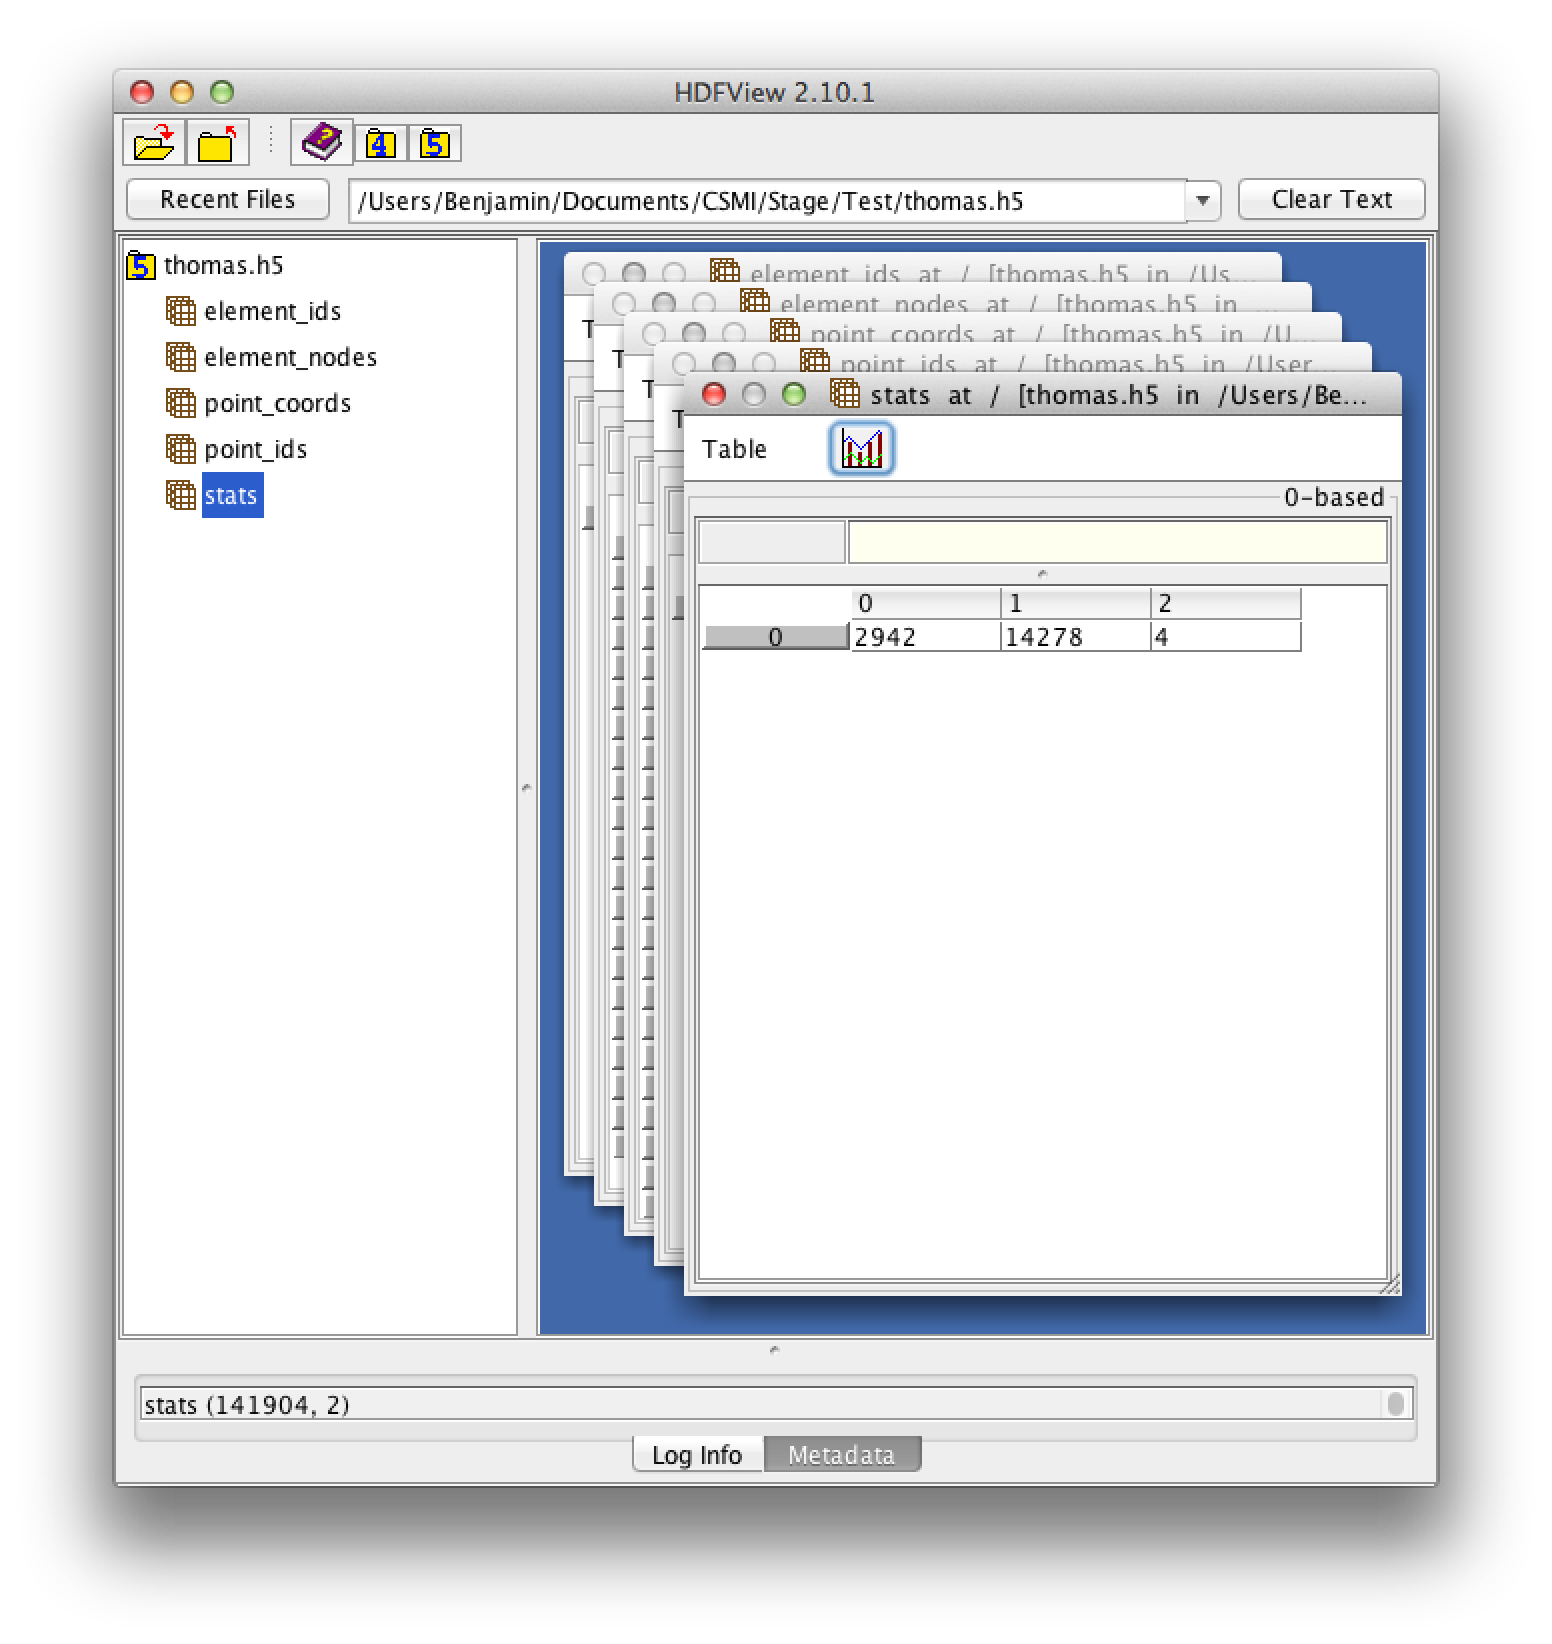
\includegraphics [width = 300pt] {HDFview.png}
\caption {HDFview}
\end {center}
\end {figure}
Une application de visualisation comme Paraview ne peut pas afficher directement les solutions contenues dans un fichier HDF5. Pour ce faire on a besoin d'un format de fichier comme XDMF de métadonnées pour rassembler les données se trouvant dans un fichier HDF5.
\newpage
\section {XDMF}
\subsection {Description}
Le XDMF (eXtensible Data Model and Format) est une librairie qui fournit un moyen d'accèder aux données contenues dans un fichier HDF5. Le language utilisé pour écrire ces métadonnées est le XML, un language à balise. L'extension de ce format de fichier est ".xmf".
\subsection {Structure d'un fichier XDMF}

Un fichier XDMF est constitué d'éléments entourées d'une balise ouvrante et fermante, et chaque élément possède zéro ou plusieurs attributs.\newline
Voici la structure d'un élément XDMF :
\begin{lstlisting}[language=XML]
<Nom element
    Nom attribut="Valeur"
    ...
</Nom element>
\end{lstlisting}
Comme tout langage à balise, un fichier XDMF commence par une entête sous cette forme :
\begin{lstlisting}[language=XML]
<?xml version="1.0" ?>
<!DOCTYPE Xdmf SYSTEM "Xdmf.dtd" []>
\end{lstlisting}
Ensuite vient le corps du fichier XDMF qui commence par la balise \emph{Xdmf} qui sert essentiellement à indiquer la version du langage :
\begin{lstlisting}[language=XML]
<Xdmf Version="2.0">
...
</Xdmf>
\end{lstlisting}
Un élément \emph{Xdmf} peut contenir un ou plusieurs éléments \emph{Domain}. Un élément \emph{Domain} peut à leur tour contenir plusieurs éléments \emph{Grid} (sous domaine de calcul). Chaque élément \emph{Grid} doivent contenir au moins un élément \emph{Geometry} (les coordonnées des points du maillage), un élément \emph{Topology} (les éléments du maillage), et zéro ou plusieurs élément \emph{Attribute} qui sert à spécifier les solutions.\newline
Les éléménts \emph{Geometry}, \emph{Topology}, \emph{Attribute} contiennent tous un élément nommé \emph{DataItem} qui indique où trouver les données correspondants.\newline
Voici un exemple : 
\begin{lstlisting}[language=XML]
<?xml version="1.0" ?>
<!DOCTYPE Xdmf SYSTEM "Xdmf.dtd" []>
  <Xdmf Version="2.0">
    <Grid>
     <Geometry>
       <DataItem Dimension="50">
         mylaplacian.h5:/points
       </DataItem>
     </Geometry>
     <Topology>
       <DataItem Dimension="102">
         mylaplacian.h5:/nodes
       </DataItem>
     </Topology>
     <Attribute>
        <DataItem Dimension="50" Center="Node">
          mylaplacian.h5:/solutions
        </DataItem>
     </Attribute>
    </Grid>
  </Xdmf>
\end{lstlisting}
\subsection {Les Attributs}
Nous détaillerons dans cette partie uniquement les attributs nécessaires à l'implémentation de notre exportateur.
\subsubsection {DataItem}
Les attributs d'un DataItem servent essentiellement à décrire les informations des données :
\begin{itemize}
\item Dimensions : indique la taille du tableau de données
\item NumberType : le type des données (Float, Int, ...)
\item Precision : la taille en octet d'un élément du tableau (1, 2, 4, ou 8 octets)
\end{itemize}
\subsubsection {Topology}
\begin{itemize}
\item TopologyType : correspond au type des éléments qui forment le maillage (triangle, piramide, ...)
\item NumberOfElement : le nombre d'éléments
\item NodesPerElement : le nombre de noeuds qui décrivent un élément
\item Dimensions : la taille du tableau de données
\end{itemize}
\subsection {L'élément Time}
Si l'on souhaite exporter des données qui varient dans le temps, il est possible de rajouter un attribut \emph{Time} dans une grille comme ceci :
\begin{lstlisting} [language=XML]
<Grid>
    <Time Value="0.5"/>
    <Geometry>
    ...
    </Geometry>
    <Topology>
    ...
    </Topology>
</Grid>
\end{lstlisting}
\newpage
Maintenant qu'on a vu la structure de ces formats de fichiers, regardons dans la suite comment exporter les données d'une simulation Feel++.
\section {Exportateur}
Le but de cet exportateur est d'exporter un maillage et les solutions sur ce maillage. Un maillage est une modélisation géométrique d'un domaine, découpé en plusieurs éléments. Un élément est composé de points, caractérisés par leurs coordonnées. 

\subsection {La classe Exporterhdf5}
L'emplacement de la classe Exporterhdf5 dans le dépôt Feel++ est le suivant : \textbf{~/feelpp/feel/feelfilters/} \newline
Dans le projet feel++, il existe déjà plusieurs exportateurs de données. Chaque classe doivent hériter de la classe principale \emph{Exporter}, pour faciliter l'instanciation d'un objet exporter en utilisant le polymorphisme du langage C++ \newline
Voici comment on sélectionne un exportateur dans la classe Exporter : 
\begin{lstlisting}
template<typename MeshType, int N>
boost::shared_ptr<Exporter<MeshType, N> >
Exporter<MeshType, N>::New( po::variables_map const& vm, std::string prefix, WorldComm const& worldComm )
{
    std::string estr = vm["exporter.format"].template as<std::string>();
    Exporter<MeshType, N>* exporter =  0;//Factory::type::instance().createObject( estr  );
    if( N > 1 && estr != "gmsh" )
        LOG(WARNING) << "[Exporter] format " << estr << " is not available for mesh order > 1 - using gmsh exporter instead\n";
    if ( N == 1 && ( estr == "ensight"   ) )
        exporter = new ExporterEnsight<MeshType, N>( worldComm );
#ifdef FEELPP_HAS_MPIIO
    else if ( N == 1 && ( estr == "ensightgold"   ) )
        exporter = new ExporterEnsightGold<MeshType, N>( worldComm );
#endif
    else if ( N == 1 && ( estr == "exodus"   ) )
        exporter = new ExporterExodus<MeshType, N>( worldComm );
    else if ( N == 1 && ( estr == "hdf5" ) )
        exporter = new Exporterhdf5<MeshType, N> ( worldComm ) ;
    else if ( N > 1 || estr == "gmsh" )
        exporter = new ExporterGmsh<MeshType,N>;
    else // fallback
        exporter = new ExporterEnsight<MeshType, N>( worldComm );

    exporter->setOptions();
    exporter->addTimeSet( timeset_ptrtype( new timeset_type( prefix ) ) );
    exporter->setPrefix( prefix );
    return boost::shared_ptr<Exporter<MeshType, N> >( exporter );
}
\end{lstlisting}
Pour utiliser notre exportateur, il faudra utiliser l'option "--exporter.format=hdf5" à l'exécution du programme.\newline
Les exportateurs devront redéfinir la méthode \emph{save} de la classe principale \emph{Exporter} car c'est à ce moment là qu'aura lieu l'écriture des données vers les fichiers.
\subsection{L'exportation du maillage}
\label{subsec:exportation}
En Feel++, il est possible d'exporter un maillage de trois manières différentes :
\begin{itemize}
\item le maillage peut être considéré comme statique en fonction du temps
\item le maillage peut changer en fonction du temps
\item le maillage peut être considéré comme statique mais dont les coordonnées des points peuvent changer 
\end{itemize}
Nous avons fait le choix de travailler dans le cas général (le premier cas), c'est à dire qu'on devra exporter le maillage pour chaque pas de temps.\newline

Pour commencer, chaque constructeur de la classe doit faire appel à la fonction init pour déterminer le type des éléments en fonction de l'ordre géométrique et de la dimension :
\begin{lstlisting}
template<typename MeshType, int N>
void
Exporterhdf5<MeshType,N>::init()
{
    if ( mesh_type::nDim == 1 )
        if ( mesh_type::Shape == SHAPE_LINE )
            M_element_type = ( mesh_type::nOrder == 1 )?"Polyline":"Edge_3";
    if ( mesh_type::nDim == 2 )
    {
        if ( mesh_type::Shape == SHAPE_TRIANGLE )
            M_element_type = ( mesh_type::nOrder == 1 )?"Triangle":"Tri_6";

        else if ( mesh_type::Shape == SHAPE_QUAD )
            M_element_type = ( mesh_type::nOrder == 1 )?"Quadrilateral":"Quad_8";
    }
    if ( mesh_type::nDim == 3 )
    {
        if ( mesh_type::Shape == SHAPE_TETRA )
            M_element_type = ( mesh_type::nOrder == 1 )?"Tetrahedron":"Tet_10";

        else if ( mesh_type::Shape == SHAPE_HEXA )
            M_element_type = ( mesh_type::nOrder == 1 )?"Hexahedron":"Hex_20";
    }
}
\end{lstlisting}
C'est en appelant la méthode \emph{write} que l'on va commencer à exporter les données vers les fichiers. Cette méthode va nous générer un fichier XDMF par processus, et autant de fichier HDF5 qu'il y a de pas de temps. Voici à quoi ressemble l'algorithme :



Le code complet de la méthode \emph{write} se trouve dans l'annexe \ref{subsec:write}.
\subsubsection{L'exportation des points}
\label{subsec:exportationpoint}
\noindent
Il faut d'abord créer un dataset dans le fichier HDF5 :
\begin{lstlisting}
M_HDF5.createTable ("point_ids", H5T_STD_U32BE, currentSpaceDims) ;
\end{lstlisting}
Ensuite on remplit le buffer de coordonnées et les identifiants des points :
\begin{lstlisting}
for (size_type i = 0 ; i < M_maxNumPoints ; i++ , pt_it++) 
{
    M_uintBuffer[i] = pt_it->id () ;
    M_realBuffer[3*i] = pt_it->node()[0] ;
    if (mesh_type::nRealDim >= 2)
        M_realBuffer[3*i + 1] = pt_it->node()[1] ;
    if (mesh_type::nRealDim >= 3)
        M_realBuffer[3*i + 2] = pt_it->node()[2] ;
}
\end{lstlisting}
On s'est rendu compte que les identifiants des points en Feel++ n'étaient pas triés, et sachant que le format XDMF ne prend pas en compte les identifiants des points, il a fallu qu'on trie ces buffers : 
\begin{lstlisting}
bubbleSort (&M_uintBuffer[0], &M_realBuffer[0], M_maxNumPoints) ;
\end{lstlisting}
Cette méthode trie à la fois deux tableaux, le premier représente les identifiants des points et le second, les coordonnées des points.
Vous trouverez le code complet du trie dans l'annexe \ref{subsec:bubbleSort}.

Les identifiants n'étant pas forcément consécutifs, il faut mémoriser donc dans un tableau de hachage pour associer les anciens identifiants au nouveaux identifiants. Cette manipulation est nécessaire pour l'exportation des éléments :
\begin{lstlisting}
for (size_type i = 0 ; i < M_maxNumPoints ; i ++) 
    M_newPointId[M_uintBuffer[i]] = i ;
\end{lstlisting}
Maintenant que le buffer est remplit, on peut désormais l' écrire dans le fichier HDF5 :
\begin{lstlisting}
M_HDF5.write ("point_ids", H5T_NATIVE_LLONG, currentSpaceDims, currentOffset , &M_uintBuffer[0]) ;
\end{lstlisting}
Enfin vient la fermeture du dataset :
\begin{lstlisting}
M_HDF5.closeTable("point_ids") ;
\end{lstlisting}
Il faut maintenant écrire la portion de code XDMF pour qu'un logiciel comme Paraview puisse retrouver les données et bien les interpréter :
\begin{lstlisting}
M_xmf << "           <Geometry GeometryType=\"XYZ\">\n" ;
M_xmf << "               <DataItem Dimensions=\"" << M_maxNumPoints << " 3\" NumberType=\"Float\" Precision=\"8\" Format=\"HDF\" Endian=\"Big\">\n" ;
M_xmf << "               " << M_fileNameStep << ".h5:/point_coords\n" ;
M_xmf << "               </DataItem>\n" ;
M_xmf << "           </Geometry>\n" ;
\end{lstlisting}
Vous trouverez le code complet de cette méthode dans l'annexe \ref{subsec:writePoint}.
\subsubsection{L'exportation des éléments}
\label{subsec:exportationelement}
Un élément est caractérisé par les identifiants des points qui le composent. C'est pourquoi il est nécessaire de connaître le nombre de points par élément et le nombre d'éléments. L'algorithme de l'exportation des éléments ressemble fortement à celui des points :
\begin{enumerate}
\item Ouverture du dataset
\begin{lstlisting}
M_HDF5.createTable ("element_nodes", H5T_STD_U32BE, currentSpacesDims) ;
\end{lstlisting}
\item Remplissage du buffer
\begin{lstlisting}
for (p_it = M_meshOut->beginParts (); k < M_numParts ;  p_it++ , k++)
{
    auto elt_it = M_meshOut->beginElementWithMarker (p_it->first) ;
    auto elt_en = M_meshOut->endElementWithMarker (p_it->first) ;
    for ( ; elt_it != elt_en ; ++elt_it , i ++)
    {
        for ( size_type j = 0 ; j < M_elementNodes ; j ++ )
            M_uintBuffer[j + M_elementNodes*i] = M_newPointId[elt_it->point(j).id()]  ; 
    }
}
\end{lstlisting}
C'est ici qu'on utilise le tableau de hachage pour récupérer les nouveaux identifiants des points.
\item \'Ecriture des données
\begin{lstlisting}
M_HDF5.write ( "element_nodes", H5T_NATIVE_LLONG, currentSpacesDims, currentOffset, &M_uintBuffer[0] ) ;
\end{lstlisting}
\item Fermeture du dataset
\begin{lstlisting}
M_HDF5.closeTable ("element_nodes") ;
\end{lstlisting}
\item \'Ecriture d'une portion XDMF associé à ces données
\begin{lstlisting}
M_xmf << "           <Topology TopologyType=\"" << M_element_type << "\" NumberOfElements=\"" << M_maxNumElements << "\" NodesPerElement=\"" << M_elementNodes << "\">\n" ;
M_xmf << "               <DataItem Dimensions=\"" <<M_maxNumElements << " " << M_elementNodes << "\" NumberType=\"Int\" Precision=\"8\" Format=\"HDF\" Endian=\"Big\">\n" ;
M_xmf << "               " << M_fileNameStep << ".h5:/element_nodes\n" ;
M_xmf << "               </DataItem>\n" ;
M_xmf << "           </Topology>\n" ;
\end{lstlisting}
\end{enumerate}
Le code complet est disponible dans l'annexe \ref{subsec:writeElement}.
\subsection{L'exportation des solutions}
Les solutions associés à un maillage peuvent être soit centrées sur les noeuds ou soit sur les éléments.
\subsubsection{Sur les noeuds}
\label{subsubsec:exportationsaveNodal}
La méthode \emph{saveNodal} prend en paramètre un itérateur sur l'ensemble des solutions sur les noeuds. L'algorithme de cette méthode est similaire encore une fois aux méthodes \emph{writePoint} et {writeElement}.\newline
En parcourant l'ensemble des solutions dans l'itérateur :\newline
On teste pour connaitre le type des données (scalaire, vectoriel, ou tenseur) pour connaitre le nombre de composantes :
\begin{lstlisting}
if ( __var->second.is_scalar )
{
    solutionName += ".scl" ; 
    attributeType = "Scalar" ;
    nComponents = 1 ;
}
else if ( __var->second.is_vectorial )
{
    solutionName += ".vec" ;
    attributeType = "Vector" ;
    nComponents = 3 ;
}
else if ( __var->second.is_tensor2 )
{
    solutionName += ".tsr" ;
    attributeType = "Tensor" ;
    nComponents = 9 ;
}
\end{lstlisting}
Création du dataset (la taille des données sont naturellement égales à celle des points) :
\begin{lstlisting}
M_HDF5.createTable (solutionName.c_str(), H5T_IEEE_F64BE, currentSpacesDims) ;
\end{lstlisting}
Ensuite il faut remplir le buffer :
\begin{lstlisting}
for ( ; p_it != p_en ; p_it++) 
{

    auto r = markedelements (M_meshOut, p_it->first, EntityProcessType::LOCAL_ONLY) ;
    auto elt_it = r.template get<1>() ;
    auto elt_en = r.template get<2>() ;

    Feel::detail::MeshPoints<float> mp ( __step->mesh().get(), elt_it, elt_en, true, true, true ) ;

    size_type e = 0 ; 

    for ( ; elt_it != elt_en ; ++elt_it )
    {
        for ( uint16_type c = 0 ; c < nComponents ; ++c )
        {
            for ( uint16_type p = 0 ; p < __step->mesh()->numLocalVertices() ; ++p, ++e )
            {
                size_type  ptid = M_newPointId[elt_it->get().point(p).id()]  ;
                size_type global_node_id = mp.ids.size()*c + ptid ;
                if ( c < __var->second.nComponents ) 
                {
                    size_type dof_id = boost::get<0>( __var->second.functionSpace()->dof()->localToGlobal ( elt_it->get().id(), p, c ) ) ;
                    M_realBuffer[global_node_id] = __var->second.globalValue ( dof_id ) ;
                }
                else
                {
                    M_realBuffer[global_node_id] = 0.0 ;
                }
            }
       
    i
}
\end{lstlisting}
La première boucle parcourt les éléments, la deuxième, les composantes des données, et la troisième les points qui forment l'élément. On fait ensuite un petit calcul pour retrouver l'indice global du tableau de données et on le stocke.\newline

Ensuite on écrit les données dans le dataset et puis on le ferme proprement :
\begin{lstlisting}
M_HDF5.write ( solutionName.c_str(), H5T_NATIVE_DOUBLE, currentSpacesDims, currentOffset, &M_realBuffer[0] ) ;
M_HDF5.closeTable (solutionName.c_str()) ; 
\end{lstlisting}
Et enfin on écrit le code XDMF associé à ce dataset :
\begin{lstlisting}
M_xmf << "           <Attribute AttributeType=\""<< attributeType << "\" Name=\"" << solutionName << "\" Center=\"Node\">\n" ;
M_xmf << "               <DataItem Dimensions=\""<< nComponents << " " << M_maxNumPoints << "\" NumberType=\"Float\" Precision=\"8\" Format=\"HDF\" Endian=\"Big\">\n" ;
M_xmf << "               "<< M_fileNameStep <<".h5:/"<< solutionName <<"\n" ;
M_xmf << "               </DataItem>\n" ;    
M_xmf << "           </Attribute>\n" ;
\end{lstlisting}
Le code complet de cette méthode se trouve dans l'annexe \ref{subsec:saveNodal}.
\subsubsection{Sur les éléments}
\label{subsubsec:exportationsaveElement}
La méthode saveElement possède quasiment la même structure que la méthode précédente. \newline
Voir l'annexe \ref{subsec:saveElement}.\newline

L'exportation de ses données peuvent durer très longtemps si le domaine est très grand, c'est pourquoi il est indispensable de paralléliser un exportateur pour accélérer le temps d'exécution.
\newpage
\section {Parallélisation}
\subsection {Première version}
Sans le dire, le code présenté jusqu'à maintenant fonctionne déjà en parallèle. Mais ce code fonctionne uniquement si l'on utilise le communicateur \emph{worldCommSeq()} MPI. L'inconvénient d'utiliser ce communicateur est que le nombre de fichier généré par l'exportateur peut être très important . En effet chaque processus aura son propre fichier XDMF et ses propres fichiers HDF5.\newline
Exemple : \newline
Si on lance un programme sur deux processus : \textbf{mpirun} -np 2 programme --exporter.format=hdf5\newline
Le nom des fichiers XDMF générés seront de la forme : programme-<nombre total de processus>\_<le rang du processus courant>.xmf\newline
Et le nom des fichiers HDF5 générés seront de la forme : programme-<nombre total de proccessus>\_<le range du precessus courant>-<le pas de temps>.h5\newline
Soit dans notre exemple : \newline
programme-2\_0.xmf\newline
programme-2\_1.xmf\newline
programme-2\_0-0.h5\newline
programme-2\_1-0.h5\newline
Si la simulation est limité à un seul pas de temps.\newline
Pour réduire le nombre de fichier généré, on utilisera une autre version qui utilise le communicateur \emph{worldComm()}.

\subsection {Deuxième version}
L'objectif de cette version est pouvoir générer un seul fichier XDMF pour les processus et un fichiers HDF5 par pas de temps. Pour faire cela, il faut qu'un seul processus pour écrire le fichier XDMF et que tous les processus écrivent dans un même fichier HDF5.\newline
Pour faciliter l'écriture des données dans le fichire HDF5, nous avons organisé en groupe, c'est-à-dire que chaque processus aura son propre groupe dans le fichier.\newline
Voici un exemple sur un programme lancé sur 5 processus :
\begin {figure}[!h]
\begin {center}
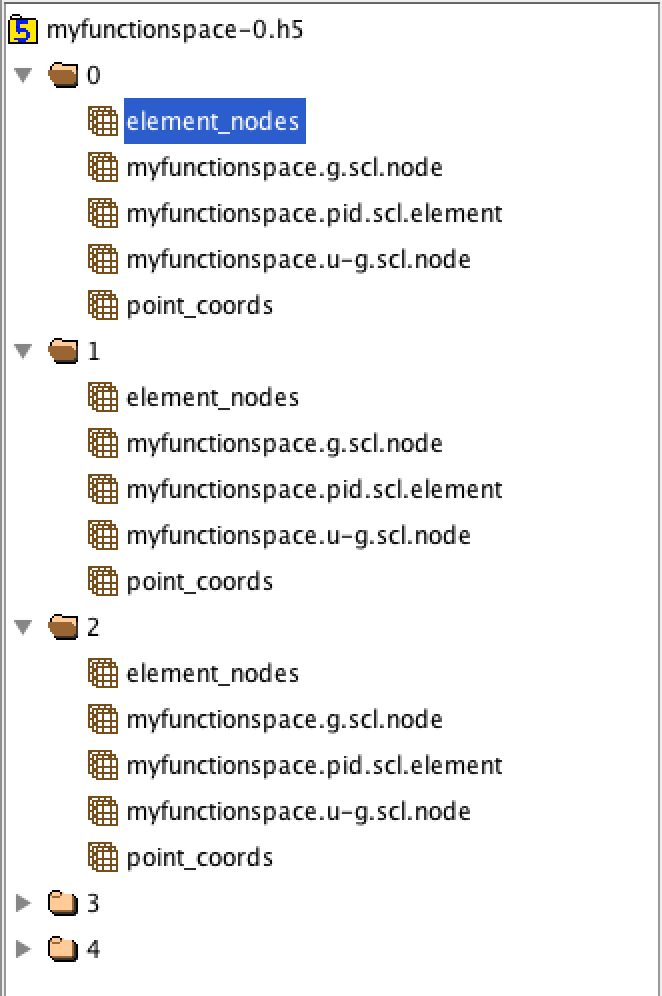
\includegraphics [width = 100pt] {HDFview5.png}
\caption {HDFview}
\end {center}
\end {figure}
\newpage
En HDF5, il faut que chaque processus crée son groupe et celui des autres, même si le processus n'écrira que dans son groupe. Il faut faire de même pour les datasets mais en plus de ça, chaque processus doit connaître la taille des datasets des autres processus. C'est pourquoi on doit utiliser un \emph{gather} MPI pour récupérer ces données.\newline
Exemple (pour l'écriture des points) :\newline
\begin{lstlisting}
std::ostringstream filestr0 ;
filestr0 << Environment::worldComm().globalRank () ;
std::vector <size_type> globalNumPoint ;
globalNumPoint.resize (Environment::worldComm().globalSize(), 0) ;
boost::mpi::all_gather(Environment::worldComm(), M_maxNumPoints, globalNumPoint) ;
for (size_type i = 0 ; i < Environment::worldComm().globalSize () ; i++)
{
    std::ostringstream filestr ;
    filestr << i  ;
    currentCount[0] = globalNumPoint[i] ;
    M_HDF5.createTable (filestr.str(), "point_coords", H5T_IEEE_F64BE, currentCount, false) ;
}
\end{lstlisting}
Il faut aussi que chaque processus ferme tous les groupes simultanément :
\begin{lstlisting}
for (size_type i = 0 ; i < Environment::worldComm().globalSize() ; i++)
{
    std::ostringstream filestr1 ;
    filestr1 << i ;
    M_HDF5.closeTable(filestr1.str()+"point_coords") ;
}
\end{lstlisting}
Pour l'écriture du fichier XDMF, seulement le processus zéro écrira le fichier. Les autres devront donc envoyer leur portion de code XDMF "Grid" au processus maître. Il existe une fonction MPI pour l'écriture en parallèle de façon ordonné en fonction du rang des processus dans un fichier.\newline
Voici un exemple : 
\begin{lstlisting}
buffer  = (char *) malloc (M_str.str().length()*sizeof(char) + 1) ;
size = M_str.str().length() ; 
M_str.str().copy (buffer, size, 0) ;
MPI_File_write_ordered (fh, buffer, size, MPI_CHAR, &status) ;
\end{lstlisting}
Il faut donner à la fonction, le type des données à transmettre, la taille du buffer, le descripteur de fichier, et le buffer de données, et MPI s'occupera de bien écrire les données dans un seul fichier.

Pour utiliser cette version, il faut ajouter l'option "--exporter.merge=true" à l'exécution du programme.
Les codes sources pour cette version sont disponibles dans l'annexe.
\newpage
\section {Conclusion}
Ce stage m'a beaucoup enrichi au niveau professionnel, en effet c'était la première que j'ai pu travailler sur un projet informatique collaboratif aussi important. L'implémentation de cet exportateur m'a permis de me familiariser avec plusieurs formats de fichiers que je ne connaissais pas pourtant très utilisés en informatique et de mieux comprendre la structure d'un maillage.\newline

Concernant le travail réalisé, l'exportateur fonctionne sur des exemples simples tel que le laplacien. Je n'ai pas testé l'exportateur sur des simulations avec des pas de temps, ni sur des simulations dont les données sont de types vectoriels. Une des perspectives sera de mettre en place l'importation que je n'ai pas pu réalisé durant ce stage faute de temps.
\newpage
\section {Annexe}
\subsection {La méthode write}
\label{subsec:write}
Retour \ref{subsec:exportation}
\begin{lstlisting}
template <typename MeshType, int N>
void Exporterhdf5<MeshType, N>::write () const 
{

    std::ostringstream str ;
    str <<  this->prefix () << "-" << Environment::worldComm().globalSize()<<"_"<<Environment::worldComm().globalRank()  ;
    M_fileName = str.str () ; 

    std::cout << "file generated                : " << M_fileName << ".xmf" << std::endl ;
    open_xdmf_xml () ;

    timeset_const_iterator __ts_it = this->beginTimeSet () ;
    timeset_const_iterator __ts_en = this->endTimeSet () ;

    timeset_ptrtype __ts = *__ts_it ;

    M_xmf << "       <Grid Name=\"Simulation over time\" GridType=\"Collection\" CollectionType=\"Temporal\">" << "\n" ;
    M_xmf << "           <Time TimeType=\"HyperSlab\">\n" ;
    M_xmf << "               <DataItem Format=\"XML\" NumberType=\"Float\" Dimensions=\"3\">\n" ;
    M_xmf << "               " << (*(__ts->beginStep()))->time() << " " << __ts->timeIncrement() << " " << __ts->numberOfTotalSteps() << "\n" ;
    M_xmf << "               </DataItem>\n" ;
    M_xmf << "           </Time>\n" ;

    while ( __ts_it != __ts_en )
    {
        __ts = *__ts_it ;
        typename timeset_type::step_const_iterator __it = __ts->beginStep () ;
        typename timeset_type::step_const_iterator __end = __ts->endStep () ;
        __it = boost::prior ( __end ) ;

        while ( __it != __end )
        {
            typename timeset_type::step_ptrtype __step = * __it ;

            if ( __step->isInMemory() )
            {
                M_meshOut = __step->mesh () ;
                std::ostringstream filestr ;
                filestr << "-" << M_step++ ;
                M_fileNameStep = M_fileName+filestr.str() ;
                M_HDF5.openFile (M_fileNameStep+".h5", Environment::worldCommSeq(), false) ;
                M_xmf << "           <Grid Name=\"" << M_fileNameStep << "\" GridType=\"Uniform\">\n" ;

                writePoints () ;
                writeElements () ;

                if ( Environment::worldCommSeq().globalRank() == Environment::worldCommSeq().masterRank() )
                {
                    //std::cout << "time                          : " << __step->time () << std::endl ; 
                    //std::cout << "time increment                : " << __ts->timeIncrement () << std::endl ; 
                    //std::cout << "numberOfSteps                 : " << __ts->numberOfSteps () << std::endl ; 
                    //std::cout << "numberOfTotalSteps            : " << __ts->numberOfTotalSteps () << std::endl ;
                    std::cout << "file generated                : " << M_fileNameStep  << ".h5" << std::endl ;
                }

                saveNodal (__step, __step->beginNodalScalar(), __step->endNodalScalar() ) ;
                saveNodal (__step, __step->beginNodalVector(), __step->endNodalVector() ) ;

                saveElement (__step, __step->beginElementScalar(), __step->endElementScalar() ) ;
                saveElement (__step, __step->beginElementVector(), __step->endElementVector() ) ;

                M_xmf << "           </Grid>\n" ;
                M_HDF5.closeFile () ;
            }
            ++__it ;
        }
        ++__ts_it ;
    }
    close_xdmf_xml () ;
    M_meshOut.reset () ;
}
\end{lstlisting}
\newpage
\subsection {La méthode bubbleSort}
\label{subsec:bubbleSort}
Retour \ref{subsec:exportationpoint}
\begin{lstlisting}
template <typename MeshType, int N>
void Exporterhdf5<MeshType, N>::bubbleSort (size_type * ids, value_type * coords, size_type n) const 
{
    size_type int_tmp ;
    value_type float_tmp ;
    bool swapped = false ;
    do 
    {
        swapped = false ;
        for (size_type j = 0 ; j < n-1 ; j ++) 
        {
            if (ids[j] > ids[j+1]) 
            {
                int_tmp = ids[j] ;
                ids[j] = ids[j+1] ;
                ids[j+1] = int_tmp ;

                float_tmp = coords[3*j] ;
                coords[3*j] = coords [3*(j+1)] ;
                coords[3*(j+1)] = float_tmp ;

                float_tmp = coords[3*j+1] ;
                coords[3*j+1] = coords [3*(j+1)+1] ;
                coords[3*(j+1)+1] = float_tmp ;

                float_tmp = coords[3*j+2] ;
                coords[3*j+2] = coords [3*(j+1)+2] ;
                coords[3*(j+1)+2] = float_tmp ;

                swapped = true ;
            }
        }
        n = n -1 ;
    }
    while (swapped) ;
}
\end{lstlisting}
\newpage
\subsection {La méthode writePoint}
\label{subsec:writePoint}
Retour \ref{subsec:exportationpoint}
\begin{lstlisting}
template <typename MeshType, int N>
void Exporterhdf5<MeshType, N>::writePoints () const 
{
    auto pt_it = M_meshOut->beginPointWithProcessId () ;
    auto const pt_en = M_meshOut->endPointWithProcessId () ;
    M_maxNumPoints= std::distance (pt_it, pt_en) ;

    hsize_t currentSpaceDims [2] ;
    hsize_t currentCount [2] ;

    currentSpaceDims[0] = 1;
    currentSpaceDims[1] = M_maxNumPoints ;

    currentCount[0] = M_maxNumPoints ;
    currentCount[1] = 3 ;

    M_HDF5.createTable ("point_coords", H5T_IEEE_F64BE, currentCount) ;
    M_HDF5.createTable ("point_ids", H5T_STD_U32BE, currentSpaceDims) ;

    M_uintBuffer.resize (currentSpaceDims[0]*currentSpaceDims[1], 0) ;
    M_realBuffer.resize (currentCount[0]*currentCount[1], 0) ;

    for (size_type i = 0 ; i < M_maxNumPoints ; i++ , pt_it++) 
    {
        M_uintBuffer[i] = pt_it->id () ;

        M_realBuffer[3*i] = pt_it->node()[0] ;
        if (mesh_type::nRealDim >= 2)
            M_realBuffer[3*i + 1] = pt_it->node()[1] ;
        if (mesh_type::nRealDim >= 3)
            M_realBuffer[3*i + 2] = pt_it->node()[2] ;
    }

    bubbleSort (&M_uintBuffer[0], &M_realBuffer[0], M_maxNumPoints) ;

    for (size_type i = 0 ; i < M_maxNumPoints ; i ++) 
        M_newPointId[M_uintBuffer[i]] = i ;

    hsize_t currentOffset[2] = {0, 0} ;

    M_HDF5.write ("point_coords", H5T_NATIVE_DOUBLE, currentCount, currentOffset, &M_realBuffer[0]) ;
    M_HDF5.write ("point_ids", H5T_NATIVE_LLONG, currentSpaceDims, currentOffset , &M_uintBuffer[0]) ;

    M_HDF5.closeTable("point_coords") ;
    M_HDF5.closeTable("point_ids") ;    
    M_xmf << "           <Geometry GeometryType=\"XYZ\">\n" ;
    M_xmf << "               <DataItem Dimensions=\"" << M_maxNumPoints << " 3\" NumberType=\"Float\" Precision=\"8\" Format=\"HDF\" Endian=\"Big\">\n" ;
    M_xmf << "               " << M_fileNameStep << ".h5:/point_coords\n" ;
    M_xmf << "               </DataItem>\n" ;
    M_xmf << "           </Geometry>\n" ;
}
\end{lstlisting}
\newpage
\subsection {La méthode writeElement}
\label{subsec:writeElement}
Retour \ref{subsec:exportationelement}
\begin{lstlisting}
template <typename MeshType, int N>
void Exporterhdf5<MeshType, N>::writeElements () const 
{
    typename mesh_type::parts_const_iterator_type p_it = M_meshOut->beginParts();
    typename mesh_type::parts_const_iterator_type p_en = M_meshOut->endParts();
    M_numParts = std::distance (p_it, p_en) ;
    M_maxNumElements = 0 ;
    for (int i = 0 ; i < M_numParts ; i++, p_it ++) 
    {
        auto elt_it = M_meshOut->beginElementWithMarker (p_it->first) ;
        auto elt_en = M_meshOut->endElementWithMarker (p_it->first) ;
        M_maxNumElements += std::distance (elt_it, elt_en) ;
    }
    M_elementNodes = M_meshOut-> numLocalVertices () ;

    hsize_t currentSpacesDims [2] ;
    hsize_t currentSpacesDims2 [2] ;

    currentSpacesDims [0] = M_maxNumElements ;
    currentSpacesDims [1] = M_elementNodes ;

    currentSpacesDims2 [0] = 1 ;
    currentSpacesDims2 [1] = M_maxNumElements ;

    M_HDF5.createTable ("element_ids", H5T_STD_U32BE, currentSpacesDims2) ;
    M_HDF5.createTable ("element_nodes", H5T_STD_U32BE, currentSpacesDims) ;

    M_uintBuffer.resize (currentSpacesDims[0]*currentSpacesDims[1], 0) ;
    std::vector<size_type> idsBuffer ;
    idsBuffer.resize (currentSpacesDims2[1], 0) ;

    M_uintBuffer.resize (currentSpacesDims[0]*currentSpacesDims[1], 0) ;

    size_type k = 0 ;
    size_type i = 0 ;
    for (p_it = M_meshOut->beginParts (); k < M_numParts ;  p_it++ , k++)
    {
        auto elt_it = M_meshOut->beginElementWithMarker (p_it->first) ;
        auto elt_en = M_meshOut->endElementWithMarker (p_it->first) ;
        for ( ; elt_it != elt_en ; ++elt_it , i ++)
        {
            idsBuffer[i] = elt_it->id () ;
            for ( size_type j = 0 ; j < M_elementNodes ; j ++ )
                M_uintBuffer[j + M_elementNodes*i] = M_newPointId[elt_it->point(j).id()]  ; 
        }
    }


    hsize_t currentOffset[2] = {0, 0} ;
    M_HDF5.write ( "element_ids", H5T_NATIVE_LLONG, currentSpacesDims2, currentOffset, &idsBuffer[0] ) ;
    M_HDF5.write ( "element_nodes", H5T_NATIVE_LLONG, currentSpacesDims, currentOffset, &M_uintBuffer[0] ) ;

    M_HDF5.closeTable ("element_ids") ;
    M_HDF5.closeTable ("element_nodes") ;

    M_xmf << "           <Topology TopologyType=\"" << M_element_type << "\" NumberOfElements=\"" << M_maxNumElements << "\" NodesPerElement=\"" << M_elementNodes << "\">\n" ;
    M_xmf << "               <DataItem Dimensions=\"" <<M_maxNumElements << " " << M_elementNodes << "\" NumberType=\"Int\" Precision=\"8\" Format=\"HDF\" Endian=\"Big\">\n" ;
    M_xmf << "               " << M_fileNameStep << ".h5:/element_nodes\n" ;
    M_xmf << "               </DataItem>\n" ;
    M_xmf << "           </Topology>\n" ;
}
\end{lstlisting}
\newpage
\subsection {La méthode saveNodal}
\label{subsec:saveNodal}
Retour \ref{subsubsec:exportationsaveNodal}
\begin{lstlisting}
template <typename MeshType, int N>
template <typename Iterator>
void Exporterhdf5<MeshType, N>::saveNodal ( typename timeset_type::step_ptrtype __step, Iterator __var, Iterator en ) const 
{   
    while ( __var != en )
    {    
        std::string attributeType ("Scalar") ;

        std::string solutionName = __var->first ;

        uint16_type nComponents = __var -> second.nComponents ;

        if ( __var->second.is_scalar )
        {
            solutionName += ".scl" ; 
            attributeType = "Scalar" ;
            nComponents = 1 ;
        }
        else if ( __var->second.is_vectorial )
        {
            solutionName += ".vec" ;
            attributeType = "Vector" ;
            nComponents = 3 ;
        }
        else if ( __var->second.is_tensor2 )
        {
            solutionName += ".tsr" ;
            attributeType = "Tensor" ;
            nComponents = 9 ;
        }

        solutionName += ".node" ;

        hsize_t currentSpacesDims [2] ;

        currentSpacesDims [0] = nComponents ;
        currentSpacesDims [1] = M_maxNumPoints ;

        M_HDF5.createTable (solutionName.c_str(), H5T_IEEE_F64BE, currentSpacesDims) ;

        M_realBuffer.resize (M_maxNumPoints*nComponents, 0) ;

        typename mesh_type::parts_const_iterator_type p_it = M_meshOut->beginParts();
        typename mesh_type::parts_const_iterator_type p_en = M_meshOut->endParts();
        M_numParts = std::distance (p_it, p_en) ;

        for ( ; p_it != p_en ; p_it++) 
        {

            auto r = markedelements (M_meshOut, p_it->first, EntityProcessType::LOCAL_ONLY) ;
            auto elt_it = r.template get<1>() ;
            auto elt_en = r.template get<2>() ;

            Feel::detail::MeshPoints<float> mp ( __step->mesh().get(), elt_it, elt_en, true, true, true ) ;

            size_type e = 0 ; 

            for ( ; elt_it != elt_en ; ++elt_it )
            {
                for ( uint16_type c = 0 ; c < nComponents ; ++c )
                {
                    for ( uint16_type p = 0 ; p < __step->mesh()->numLocalVertices() ; ++p, ++e )
                    {
                        size_type  ptid = M_newPointId[elt_it->get().point(p).id()]  ;
                        size_type global_node_id = mp.ids.size()*c + ptid ;
                        if ( c < __var->second.nComponents ) 
                        {
                            size_type dof_id = boost::get<0>( __var->second.functionSpace()->dof()->localToGlobal ( elt_it->get().id(), p, c ) ) ;
                            M_realBuffer[global_node_id] = __var->second.globalValue ( dof_id ) ;
                        }
                        else
                        {
                            M_realBuffer[global_node_id] = 0.0 ;
                        }
                    }
                }
            }
        }    
        hsize_t currentOffset[2] = {0, 0} ;

        M_HDF5.write ( solutionName.c_str(), H5T_NATIVE_DOUBLE, currentSpacesDims, currentOffset, &M_realBuffer[0] ) ;

        M_HDF5.closeTable (solutionName.c_str()) ;    

        M_xmf << "           <Attribute AttributeType=\""<< attributeType << "\" Name=\"" << solutionName << "\" Center=\"Node\">\n" ;
        M_xmf << "               <DataItem Dimensions=\""<< nComponents << " " << M_maxNumPoints << "\" NumberType=\"Float\" Precision=\"8\" Format=\"HDF\" Endian=\"Big\">\n" ;
        M_xmf << "               "<< M_fileNameStep <<".h5:/"<< solutionName <<"\n" ;
        M_xmf << "               </DataItem>\n" ;    
        M_xmf << "           </Attribute>\n" ;
        ++__var ;
    }
}
\end{lstlisting}
\newpage
\subsection {La méthode saveElement}
\label{subsec:saveElement}
Retour \ref{subsubsec:exportationsaveElement}
\begin{lstlisting}
template<typename MeshType, int N>
template<typename Iterator>
void Exporterhdf5<MeshType, N>::saveElement ( typename timeset_type::step_ptrtype __step, Iterator __evar, Iterator __evaren ) const 
{
    while ( __evar != __evaren ) 
    {
        std::string attributeType ("Scalar") ;

        std::string solutionName = __evar->first ;
        uint16_type nComponents = __evar->second.nComponents ;

        if ( __evar->second.is_scalar )
        {
            solutionName += ".scl" ; 
            attributeType = "Scalar" ;
            nComponents = 1 ;
        }
        else if ( __evar->second.is_vectorial )
        {
            solutionName += ".vec" ;
            attributeType = "Vector" ;
            nComponents = 3 ;
        }
        else if ( __evar->second.is_tensor2 )
        {
            solutionName += ".tsr" ;
            attributeType = "Tensor" ;
            nComponents = 9 ;
        }
        solutionName += ".element" ;
        hsize_t currentSpacesDims [2] ;

        currentSpacesDims [0] = nComponents ;
        currentSpacesDims [1] = M_maxNumElements ;

        M_HDF5.createTable (solutionName.c_str(), H5T_IEEE_F64BE, currentSpacesDims) ;

        M_realBuffer.resize (M_maxNumElements*nComponents, 0) ;

        typename mesh_type::parts_const_iterator_type p_it = M_meshOut->beginParts() ;
        typename mesh_type::parts_const_iterator_type p_en = M_meshOut->endParts() ;
        for ( ; p_it != p_en ; p_it++ ) 
        {
            typename mesh_type::marker_element_const_iterator elt_st ;
            typename mesh_type::marker_element_const_iterator elt_en ;
            boost::tie( elt_st, elt_en ) = __step->mesh()->elementsWithMarker( p_it->first, __evar->second.worldComm().localRank() ) ;

            if ( !__evar->second.areGlobalValuesUpdated() )
                __evar->second.updateGlobalValues() ;

            size_type ncells = std::distance ( elt_st, elt_en ) ;
            for ( int c = 0 ; c < nComponents ; ++c )
            {
                size_type e = 0 ;
                for ( auto elt_it = elt_st ; elt_it != elt_en ; ++elt_it, ++e )
                {
                    size_type global_node_id = c*ncells+e ;
                    if ( c < __evar->second.nComponents )
                    {
                        size_type dof_id = boost::get<0>( __evar->second.functionSpace()->dof()->localToGlobal( elt_it->id(), 0, c ) ) ;
                        M_realBuffer[global_node_id] = __evar->second.globalValue ( dof_id ) ;
                    }
                    else 
                        M_realBuffer[global_node_id] = 0 ;
                }
            }
        }   
        hsize_t currentOffset[2] = {0, 0} ;

        M_HDF5.write ( solutionName.c_str(), H5T_NATIVE_DOUBLE, currentSpacesDims, currentOffset, &M_realBuffer[0] ) ;

        M_HDF5.closeTable (solutionName.c_str()) ;    

        M_xmf << "           <Attribute AttributeType=\"" << attributeType << "\" Name=\"" << solutionName << "\" Center=\"Cell\">\n" ;
        M_xmf << "               <DataItem Dimensions=\""<< nComponents <<" "<< M_maxNumElements << "\" NumberType=\"Float\" Precision=\"8\" Format=\"HDF\" Endian=\"Big\">\n" ;
        M_xmf << "               "<< M_fileNameStep << ".h5:/" << solutionName << "\n" ;
        M_xmf << "               </DataItem>\n" ;    
        M_xmf << "           </Attribute>\n" ;
        __evar++ ;
    }
}
\end{lstlisting}
\newpage
\subsection {La méthode save}
\begin{lstlisting}
template <typename MeshType, int N>
void Exporterhdf5<MeshType, N>::save () const 
{
    if ( Environment::worldComm().globalRank() == Environment::worldComm().masterRank() )
        std::cout << "exporter.merge                : " << (boption (_name = "exporter.merge" ) ? "true" : "false")  << std::endl ;
    if ( boption ( _name = "exporter.merge" ) )
        writeMerge() ;
    else 
        write () ;
}
\end{lstlisting}
\newpage
\subsection {La méthode writeMerge}
\begin{lstlisting}
template <typename MeshType, int N>
void Exporterhdf5<MeshType, N>::writeMerge () const 
{

    MPI_Status status;
    int size ;
    M_str <<  this->prefix () << ".xmf" ;
    M_fileName = M_str.str () ; 

    char * strTmp = strdup (M_fileName.c_str()) ;
    if(this->worldComm().isMasterRank() && fs::exists(strTmp))
    {
        MPI_File_delete(strTmp, MPI_INFO_NULL);
    }
    MPI_Barrier( Environment::worldComm().comm() );
    MPI_File_open( this->worldComm().comm(), strTmp, MPI_MODE_RDWR | MPI_MODE_CREATE, MPI_INFO_NULL, &fh );
    free (strTmp) ;

    size_type rank = Environment::worldComm().globalRank () ;

    timeset_const_iterator __ts_it = this->beginTimeSet () ;
    timeset_const_iterator __ts_en = this->endTimeSet () ;

    timeset_ptrtype __ts = *__ts_it ;

    M_str.str("") ;
    M_str << "<?xml version=\"1.0\" ?>\n" ;
    M_str << "<!DOCTYPE Xdmf SYSTEM \"Xdmf.dtd\" []>\n" ;
    M_str << "<Xdmf Version=\"2.0\">\n" ;
    M_str << "   <Domain>\n" ;
    M_str << "       <Grid Name=\"Simulation\" GridType=\"Collection\" CollectionType=\"Spatial\">\n" ;

    char * buffer  = (char *) malloc (M_str.str().length()*sizeof(char) + 1) ;
    if ( this->worldComm().isMasterRank() ) 
    { size = M_str.str().length() ; }
    else
    { size = 0 ; }
    M_str.str().copy (buffer, size, 0) ;
    MPI_File_write_ordered (fh, buffer, size, MPI_CHAR, &status) ;

    if ( Environment::worldComm().globalRank() == Environment::worldComm().masterRank() )
        std::cout << "file generated                : " << M_fileName << std::endl ;

    while ( __ts_it != __ts_en )
    {
        __ts = *__ts_it ;
        typename timeset_type::step_const_iterator __it = __ts->beginStep () ;
        typename timeset_type::step_const_iterator __end = __ts->endStep () ;
        __it = boost::prior ( __end ) ;

        while ( __it != __end )
        {
            typename timeset_type::step_ptrtype __step = * __it ;

            if ( __step->isInMemory() )
            {
                M_meshOut = __step->mesh () ;
                std::ostringstream filestr ;
                filestr << "-" << M_step++ ;
                M_fileNameStep = this->prefix() + filestr.str() ;
                M_HDF5.openFile (M_fileNameStep+".h5", Environment::worldComm(), false) ;

                M_str.str("") ;
                M_str << "           <Grid Name=\"" << M_fileNameStep << "\" GridType=\"Uniform\">\n" ;
                M_str << "               <Time Value=\"" << __step->time() << "\"/>\n" ;  

                writePointsMerge () ;
                writeElementsMerge () ;

                if ( Environment::worldComm().globalRank() == Environment::worldComm().masterRank() )
                {
                    //std::cout << "time                          : " << __step->time () << std::endl ; 
                    //std::cout << "time increment                : " << __ts->timeIncrement () << std::endl ; 
                    //std::cout << "numberOfSteps                 : " << __ts->numberOfSteps () << std::endl ; 
                    //std::cout << "numberOfTotalSteps            : " << __ts->numberOfTotalSteps () << std::endl ;
                    std::cout << "file generated                : " << M_fileNameStep  << ".h5" << std::endl ;
                }

                saveNodalMerge (__step, __step->beginNodalScalar(), __step->endNodalScalar() ) ;
                saveNodalMerge (__step, __step->beginNodalVector(), __step->endNodalVector() ) ;

                saveElementMerge (__step, __step->beginElementScalar(), __step->endElementScalar() ) ;
                saveElementMerge (__step, __step->beginElementVector(), __step->endElementVector() ) ;

                M_str << "           </Grid>\n" ;
                free (buffer) ;
                buffer  = (char *) malloc (M_str.str().length()*sizeof(char) + 1) ;
                size = M_str.str().length() ; 
                M_str.str().copy (buffer, size, 0) ;
                MPI_File_write_ordered (fh, buffer, size, MPI_CHAR, &status) ;

                M_HDF5.closeFile () ;
            }
            ++__it ;
        }
        ++__ts_it ;
    }
    M_str.str("") ;
    M_str << "       </Grid>\n" ;
    M_str << "   </Domain>\n" ;
    M_str << "</Xdmf>\n"  ;

    free (buffer) ;
    buffer  = (char *) malloc (M_str.str().length()*sizeof(char) + 1) ;
    if ( this->worldComm().isMasterRank() ) 
    { size = M_str.str().length() ; }
    else
    { size = 0 ; }
    M_str.str().copy (buffer, size, 0) ;
    MPI_File_write_ordered (fh, buffer, size, MPI_CHAR, &status) ;

    MPI_File_close(&fh) ;
    free (buffer) ;
}
\end{lstlisting}
\newpage
\subsection {La méthode writePointMerge}
\begin{lstlisting}
template <typename MeshType, int N>
void Exporterhdf5<MeshType, N>::writePointsMerge () const 
{
    auto pt_it = M_meshOut->beginPointWithProcessId () ;
    auto const pt_en = M_meshOut->endPointWithProcessId () ;
    M_maxNumPoints= std::distance (pt_it, pt_en) ;

    hsize_t currentSpaceDims [2] ;
    hsize_t currentCount [2] ;

    currentSpaceDims[0] = 1;
    currentSpaceDims[1] = M_maxNumPoints ;

    currentCount[0] = M_maxNumPoints ;
    currentCount[1] = 3 ;
    std::ostringstream filestr0 ;
    filestr0 << Environment::worldComm().globalRank () ;
    std::vector <size_type> globalNumPoint ;
    globalNumPoint.resize (Environment::worldComm().globalSize(), 0) ;
    boost::mpi::all_gather(Environment::worldComm(), M_maxNumPoints, globalNumPoint) ;
    for (size_type i = 0 ; i < Environment::worldComm().globalSize () ; i++)
    {
        std::ostringstream filestr ;
        filestr << i  ;
        currentCount[0] = globalNumPoint[i] ;
        M_HDF5.createTable (filestr.str(), "point_coords", H5T_IEEE_F64BE, currentCount, false) ;
    }
    currentCount[0] = M_maxNumPoints ;
    M_uintBuffer.resize (currentSpaceDims[0]*currentSpaceDims[1], 0) ;
    M_realBuffer.resize (currentCount[0]*currentCount[1], 0) ;

    for (size_type i = 0 ; i < M_maxNumPoints ; i++ , pt_it++) 
    {
        M_uintBuffer[i] = pt_it->id () ;

        M_realBuffer[3*i] = pt_it->node()[0] ;
        if (mesh_type::nRealDim >= 2)
            M_realBuffer[3*i + 1] = pt_it->node()[1] ;
        if (mesh_type::nRealDim >= 3)
            M_realBuffer[3*i + 2] = pt_it->node()[2] ;
    }

    bubbleSort (&M_uintBuffer[0], &M_realBuffer[0], M_maxNumPoints) ;

    for (size_type i = 0 ; i < M_maxNumPoints ; i ++) 
        M_newPointId[M_uintBuffer[i]] = i ;

    hsize_t currentOffset[2] = {0, 0} ;

    Environment::worldComm().barrier() ;
    M_HDF5.write (filestr0.str()+"point_coords", H5T_NATIVE_DOUBLE, currentCount, currentOffset, &M_realBuffer[0]) ;
    Environment::worldComm().barrier() ;

    for (size_type i = 0 ; i < Environment::worldComm().globalSize() ; i++)
    {
        std::ostringstream filestr1 ;
        filestr1 << i ;
        M_HDF5.closeTable(filestr1.str()+"point_coords") ;
    }

    M_str << "               <Geometry GeometryType=\"XYZ\">\n" ;
    M_str << "                   <DataItem Dimensions=\"" << M_maxNumPoints << " 3\" NumberType=\"Float\" Precision=\"8\" Format=\"HDF\" Endian=\"Big\">\n" ;
    M_str << "                   " << M_fileNameStep << ".h5:/" << filestr0.str() << "/point_coords\n" ;
    M_str << "                   </DataItem>\n" ;
    M_str << "               </Geometry>\n" ;
}
\end{lstlisting}
\newpage
\subsection {La méthode writeElementMerge}
\begin{lstlisting}
template <typename MeshType, int N>
void Exporterhdf5<MeshType, N>::writeElementsMerge () const 
{
    typename mesh_type::parts_const_iterator_type p_it = M_meshOut->beginParts();
    typename mesh_type::parts_const_iterator_type p_en = M_meshOut->endParts();
    M_numParts = std::distance (p_it, p_en) ;
    M_maxNumElements = 0 ;
    for (int i = 0 ; i < M_numParts ; i++, p_it ++) 
    {
        auto elt_it = M_meshOut->beginElementWithMarker (p_it->first) ;
        auto elt_en = M_meshOut->endElementWithMarker (p_it->first) ;
        M_maxNumElements += std::distance (elt_it, elt_en) ;
    }
    M_elementNodes = M_meshOut-> numLocalVertices () ;

    hsize_t currentSpacesDims [2] ;
    hsize_t currentSpacesDims2 [2] ;

    currentSpacesDims [0] = M_maxNumElements ;
    currentSpacesDims [1] = M_elementNodes ;

    currentSpacesDims2 [0] = 1 ;
    currentSpacesDims2 [1] = M_maxNumElements ;

    std::ostringstream filestr0 ;
    filestr0 << Environment::worldComm().globalRank () ;
    std::vector <size_type> globalNumElements ;
    globalNumElements.resize (Environment::worldComm().globalSize(), 0) ;
    boost::mpi::all_gather(Environment::worldComm(), M_maxNumElements, globalNumElements) ;

    for (size_type i = 0 ; i < Environment::worldComm().globalSize () ; i++)
    {
        std::ostringstream filestr ;
        filestr << i  ;
        currentSpacesDims [0] = globalNumElements[i] ;

        M_HDF5.createTable (filestr.str(), "element_nodes", H5T_STD_U32BE, currentSpacesDims, true) ;
    }
    currentSpacesDims [0] = M_maxNumElements ;

    M_uintBuffer.resize (currentSpacesDims[0]*currentSpacesDims[1], 0) ;
    std::vector<size_type> idsBuffer ;
    idsBuffer.resize (currentSpacesDims2[1], 0) ;

    M_uintBuffer.resize (currentSpacesDims[0]*currentSpacesDims[1], 0) ;

    size_type k = 0 ;
    size_type i = 0 ;
    for (p_it = M_meshOut->beginParts (); k < M_numParts ;  p_it++ , k++)
    {
        auto elt_it = M_meshOut->beginElementWithMarker (p_it->first) ;
        auto elt_en = M_meshOut->endElementWithMarker (p_it->first) ;
        for ( ; elt_it != elt_en ; ++elt_it , i ++)
        {
            idsBuffer[i] = elt_it->id () ;
            for ( size_type j = 0 ; j < M_elementNodes ; j ++ )
                M_uintBuffer[j + M_elementNodes*i] = M_newPointId[elt_it->point(j).id()]  ; 
        }
    }


    hsize_t currentOffset[2] = {0, 0} ;
    M_HDF5.write ( filestr0.str()+"element_nodes", H5T_NATIVE_LLONG, currentSpacesDims, currentOffset, &M_uintBuffer[0] ) ;

    for (size_type i = 0 ; i < Environment::worldComm().globalSize() ; i++)
    {
        std::ostringstream filestr1 ;
        filestr1 << i ;
        M_HDF5.closeTable(filestr1.str()+"element_nodes") ;
    }
    M_str << "               <Topology TopologyType=\"" << M_element_type << "\" NumberOfElements=\"" << M_maxNumElements << "\" NodesPerElement=\"" << M_elementNodes << "\">\n" ;
    M_str << "                   <DataItem Dimensions=\"" <<M_maxNumElements << " " << M_elementNodes << "\" NumberType=\"Int\" Precision=\"8\" Format=\"HDF\" Endian=\"Big\">\n" ;
    M_str << "                   " << M_fileNameStep << ".h5:/" << filestr0.str() << "/element_nodes\n" ;
    M_str << "                   </DataItem>\n" ;
    M_str << "               </Topology>\n" ;
}
\end{lstlisting}
\newpage
\subsection {La méthode saveNodalMerge}
\begin{lstlisting}
template <typename MeshType, int N>
template <typename Iterator>
void Exporterhdf5<MeshType, N>::saveNodalMerge ( typename timeset_type::step_ptrtype __step, Iterator __var, Iterator en ) const 
{   
    while ( __var != en )
    {    
        std::string attributeType ("Scalar") ;

        std::string solutionName = __var->first ;

        uint16_type nComponents = __var -> second.nComponents ;

        if ( __var->second.is_scalar )
        {
            solutionName += ".scl" ; 
            attributeType = "Scalar" ;
            nComponents = 1 ;
        }
        else if ( __var->second.is_vectorial )
        {
            solutionName += ".vec" ;
            attributeType = "Vector" ;
            nComponents = 3 ;
        }
        else if ( __var->second.is_tensor2 )
        {
            solutionName += ".tsr" ;
            attributeType = "Tensor" ;
            nComponents = 9 ;
        }

        solutionName += ".node" ;

        //        if ( Environment::worldComm().globalRank() == Environment::worldComm().masterRank() )
        //            std::cout << "solution name                 : " << solutionName << std::endl ;

        hsize_t currentSpacesDims [2] ;

        currentSpacesDims [0] = nComponents ;
        currentSpacesDims [1] = M_maxNumPoints ;

        std::ostringstream filestr0 ;
        filestr0 << Environment::worldComm().globalRank () ;

        std::vector <size_type> globalNumPoint ;
        globalNumPoint.resize (Environment::worldComm().globalSize(), 0) ;
        boost::mpi::all_gather(Environment::worldComm(), M_maxNumPoints, globalNumPoint) ;

        for (size_type i = 0 ; i < Environment::worldComm().globalSize () ; i++)
        {
            std::ostringstream filestr ;
            filestr << i  ;
            currentSpacesDims [1] = globalNumPoint[i] ;

            M_HDF5.createTable (filestr.str(), solutionName.c_str() , H5T_IEEE_F64BE, currentSpacesDims, true) ;
        }

        currentSpacesDims [1] = M_maxNumPoints ;

        M_realBuffer.resize (M_maxNumPoints*nComponents, 0) ;

        typename mesh_type::parts_const_iterator_type p_it = M_meshOut->beginParts();
        typename mesh_type::parts_const_iterator_type p_en = M_meshOut->endParts();
        M_numParts = std::distance (p_it, p_en) ;

        for ( ; p_it != p_en ; p_it++) 
        {

            auto r = markedelements (M_meshOut, p_it->first, EntityProcessType::LOCAL_ONLY) ;
            auto elt_it = r.template get<1>() ;
            auto elt_en = r.template get<2>() ;

            Feel::detail::MeshPoints<float> mp ( __step->mesh().get(), elt_it, elt_en, true, true, true ) ;

            size_type e = 0 ; 

            for ( ; elt_it != elt_en ; ++elt_it )
            {
                for ( uint16_type c = 0 ; c < nComponents ; ++c )
                {
                    for ( uint16_type p = 0 ; p < __step->mesh()->numLocalVertices() ; ++p, ++e )
                    {
                        size_type  ptid = M_newPointId[elt_it->get().point(p).id()]  ;
                        size_type global_node_id = mp.ids.size()*c + ptid ;
                        if ( c < __var->second.nComponents ) 
                        {
                            size_type dof_id = boost::get<0>( __var->second.functionSpace()->dof()->localToGlobal ( elt_it->get().id(), p, c ) ) ;
                            M_realBuffer[global_node_id] = __var->second.globalValue ( dof_id ) ;
                        }
                        else
                        {
                            M_realBuffer[global_node_id] = 0.0 ;
                        }
                    }
                }
            }
        }    
        hsize_t currentOffset[2] = {0, 0} ;

        M_HDF5.write ( filestr0.str() + solutionName, H5T_NATIVE_DOUBLE, currentSpacesDims, currentOffset, &M_realBuffer[0] ) ;

        for (size_type i = 0 ; i < Environment::worldComm().globalSize() ; i++)
        {
            std::ostringstream filestr1 ;
            filestr1 << i ;
            M_HDF5.closeTable(filestr1.str()+solutionName) ;
        }

        M_str << "               <Attribute AttributeType=\""<< attributeType << "\" Name=\"" << solutionName << "\" Center=\"Node\">\n" ;
        M_str << "                   <DataItem Dimensions=\""<< nComponents << " " << M_maxNumPoints << "\" NumberType=\"Float\" Precision=\"8\" Format=\"HDF\" Endian=\"Big\">\n" ;
        M_str << "                   "<< M_fileNameStep <<".h5:/"<< filestr0.str() << "/" <<solutionName <<"\n" ;
        M_str << "                   </DataItem>\n" ;    
        M_str << "               </Attribute>\n" ;
        ++__var ;
    }
}
\end{lstlisting}
\end{document}








